\documentclass[12pt]{article}
\usepackage{amsmath}
\usepackage{graphicx}
\usepackage{float}
\usepackage{subfigure}
\usepackage{setspace}
\usepackage{amssymb}
\usepackage[backend=biber, style=authoryear]{biblatex}
\usepackage{enumerate}
\usepackage{multirow}
\usepackage{caption}
\usepackage{hyperref}
\usepackage{booktabs}
\usepackage{geometry}
\usepackage{xcolor}

% Set page margins
\geometry{margin=1in}

% Set single spacing
\singlespacing



\title{Feature Selection and Ensemble Learning for Alzheimer's Disease Prediction}
\author{R11323024 Fan Wei-Yu}
\date{April 9, 2024}
\addbibresource{reference.bib}
\begin{document}
\maketitle

\section{Introduction}
Alzheimer's disease (AD) is a progressive neurodegenerative disorder that affects memory, cognition, and behavior. Early diagnosis is crucial for effective treatment and care planning. This study aims to develop and evaluate machine learning models for predicting Alzheimer's disease based on demographic, clinical, and behavioral features.

\section{Data Description}
\label{sec:data}

The Alzheimer's disease dataset used in this study contains clinical and demographic data from patients. The dataset includes the following key features:

\begin{itemize}
    \item Demographic features: Age, Gender, Education Level, Ethnicity
    \item Clinical measurements: Blood pressure, cholesterol levels (Total, LDL, HDL, Triglycerides)
    \item Risk factors: Smoking, Alcohol consumption, BMI, Physical activity, etc.
    \item Cognitive assessments: MMSE (Mini-Mental State Examination), Functional Assessment, ADL (Activities of Daily Living)
    \item Behavioral indicators: Memory complaints, Behavioral problems, Confusion, etc.
    \item Target variable: Diagnosis (binary classification: has Alzheimer's or not)
\end{itemize}

Initial data exploration revealed a relatively balanced dataset with minimal missing values. It shows the ratio of "Alzheimer's diagnosis" is Positive : Negative = 760:1389.

Feature correlation analysis identified strong relationships between several predictors and the target variable. The most significant correlations were observed between cognitive assessments (MMSE, Functional Assessment, ADL), behavioral indicators (Behavioral Problems, Memory Complaints), and Alzheimer's diagnosis, as shown in Figure \ref{fig:correlation}.

\begin{figure}[H]
    \centering
    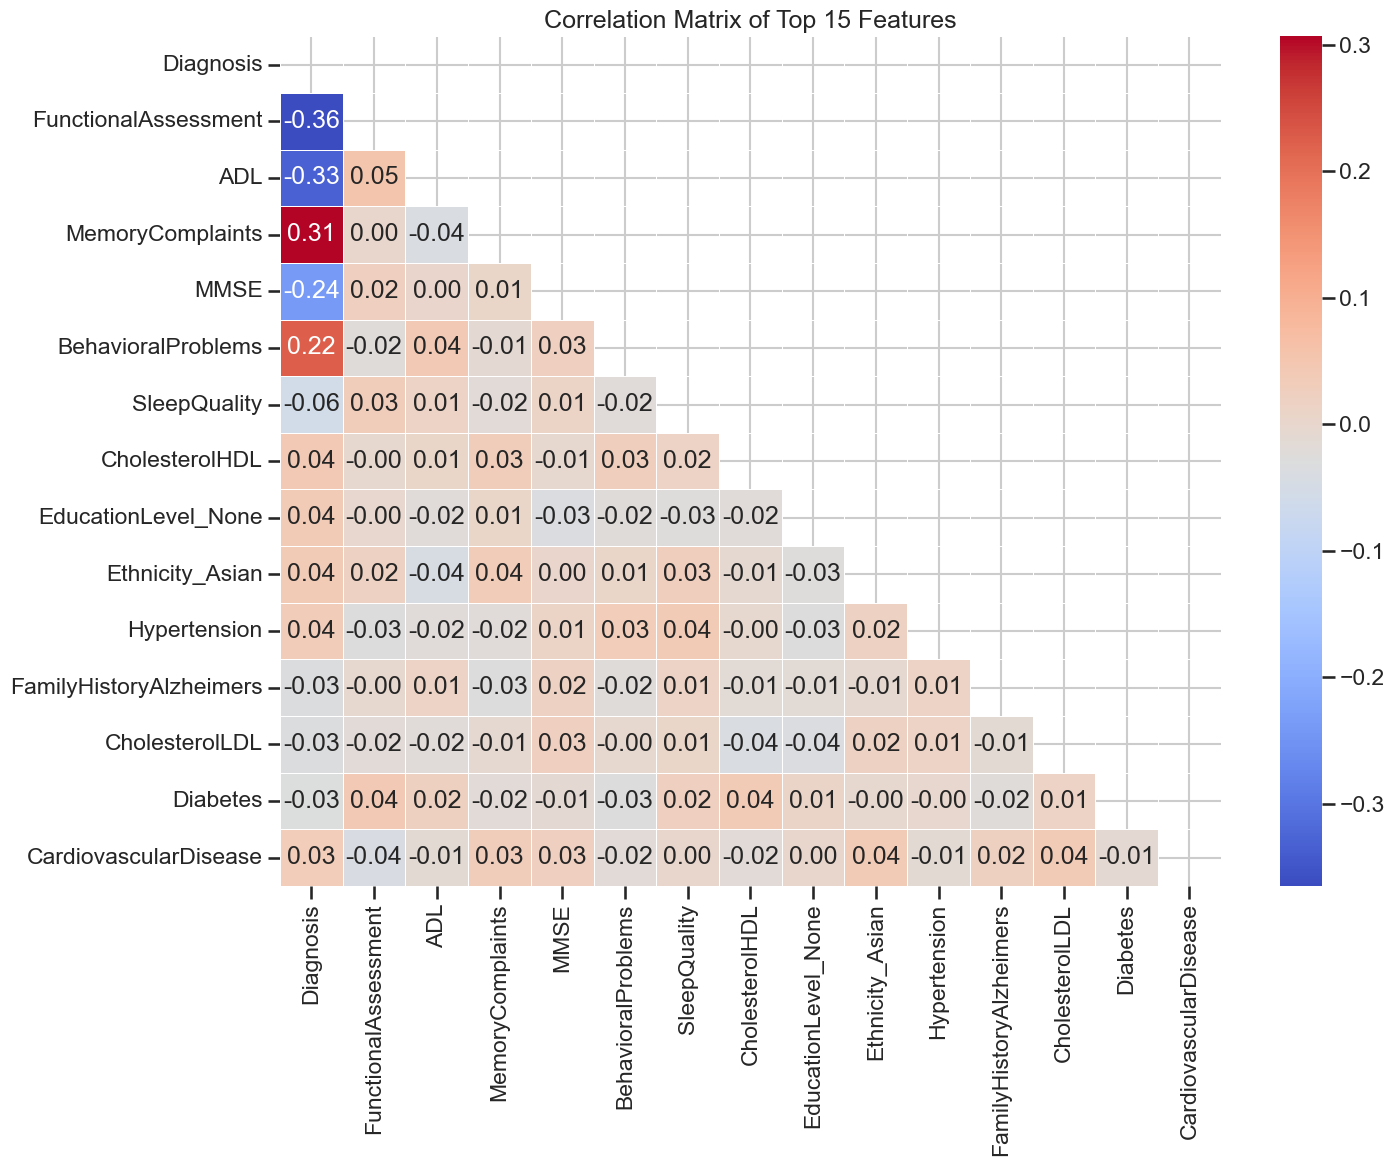
\includegraphics[width=0.85\textwidth]{figures/correlation_heatmap.png}
    \caption{Correlation Matrix of Top Correlated Features with Alzheimer's Diagnosis}
    \label{fig:correlation}
\end{figure}

\section{Classification Methods}
\label{sec:methods}

Three classification methods were implemented and compared for predicting Alzheimer's disease:

\subsection{Logistic Regression}
Logistic regression was implemented with L2 regularization. Hyperparameter tuning was performed using grid search with 5-fold cross-validation. The inverse regularization strength (C) and solver algorithm were optimized to achieve the best performance.

\subsection{Random Forest}
A random forest classifier was trained with hyperparameter tuning for the number of estimators, maximum depth, and minimum samples required for a split. This ensemble method combines multiple decision trees to improve prediction accuracy and reduce overfitting.

\subsection{XGBoost}
XGBoost (eXtreme Gradient Boosting) was implemented with optimized hyperparameters including maximum depth, gamma, subsample ratio, and column sample ratio. This gradient boosting framework is known for its efficiency and performance in classification tasks.

\subsection{Model Selection and Evaluation}
For each method, hyperparameter tuning was performed using grid search with 5-fold cross-validation. Models were evaluated using multiple metrics including accuracy, precision, recall, F1-score, and ROC-AUC. Table \ref{tab:model_comparison} presents the comparative performance of all three models.

\begin{table}[H]
    \centering
    \caption{Performance Comparison of Classification Models}
    \label{tab:model_comparison}
    \begin{tabular}{lccccc}
        \toprule
        \textbf{Model} & \textbf{Accuracy} & \textbf{Precision} & \textbf{Recall} & \textbf{F1-Score} & \textbf{ROC-AUC} \\
        \midrule
        Logistic Regression & 82.79\%&78.42\%&71.24\%&74.66\%&89.36\% \\
        Random Forest & 93.72\% & 96.32\% & 85.62\% & 90.66\% & 94.73\% \\
        XGBoost & 94.88\% &95.17\% & 90.20\% & 92.62\% & 94.50\% \\
        \bottomrule
    \end{tabular}
\end{table}

All three models demonstrated strong performance in predicting Alzheimer's disease, with XGBoost slightly outperforming the others on accuracy.

\begin{figure}[H]
    \centering
    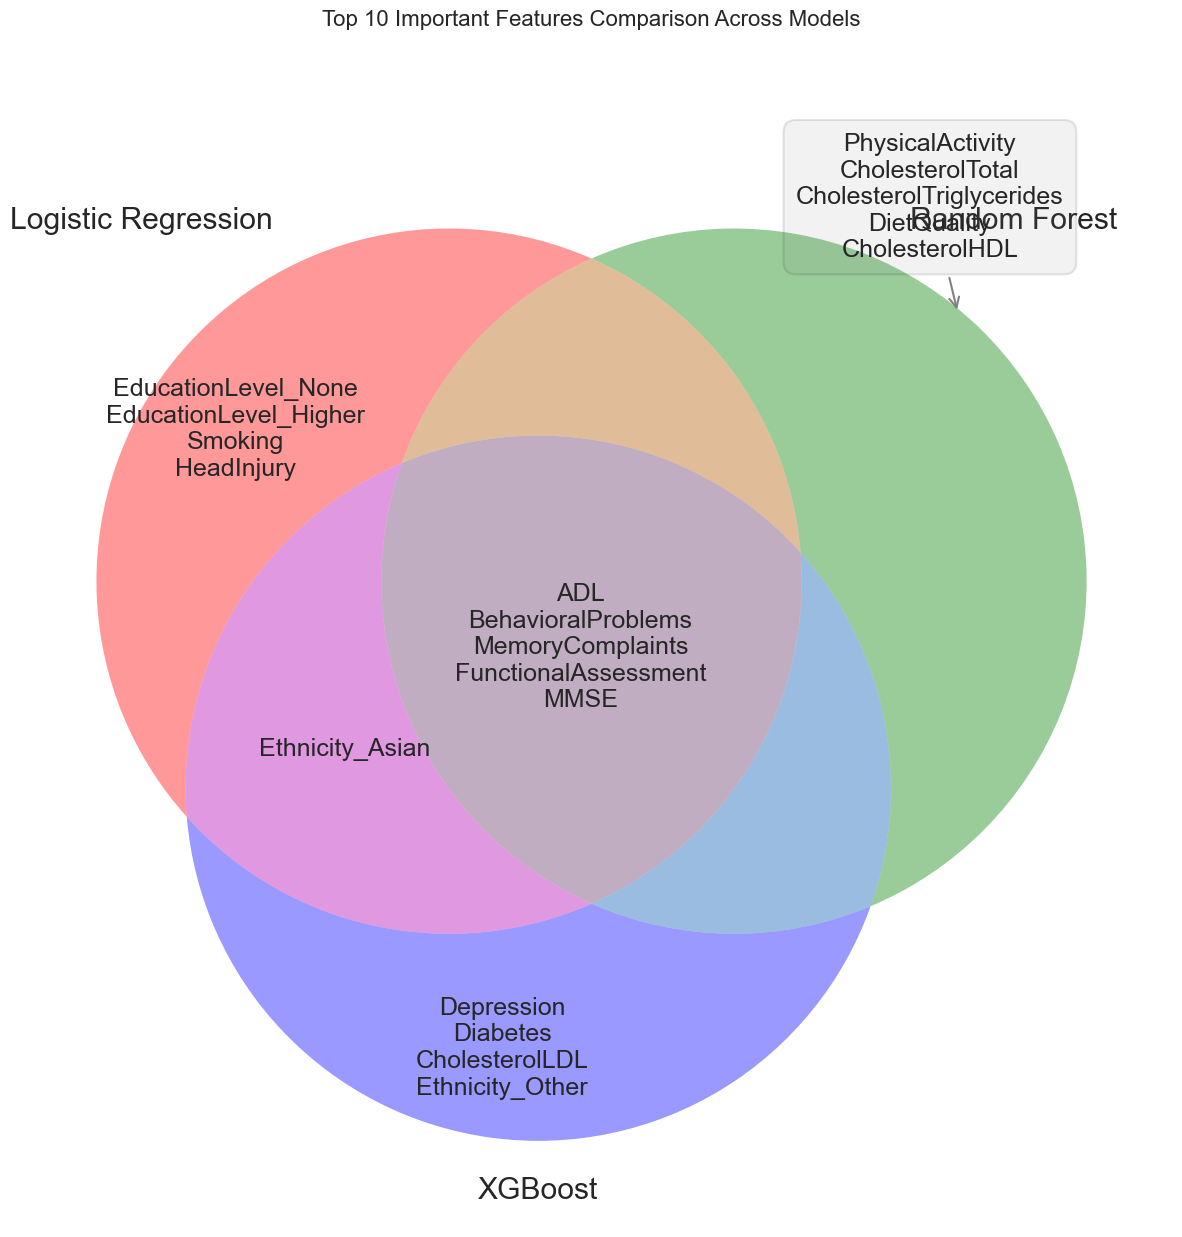
\includegraphics[width=0.5\textwidth]{figures/top10features_venns.png}
    \caption{The importance of XGBoost and Random Forest is defined by total information gain, while Logistic Regression is defined by the absolute value of the coefficients.}
    \label{fig:feature_importance}
\end{figure}

\section{Further Analysis}
\label{sec:further}

\subsection{Feature Importance Analysis}
Feature importance was analyzed across all three models to identify the most predictive features for Alzheimer's disease. Figure \ref{fig:feature_importance} shows the top features identified by each model.



Interestingly, all three models identified similar sets of important features, which are MMSE, Functional Assessment, ADL,Memory Complaints, and Behavioral Problems. The resault is consistent with figure \ref{fig:correlation}.

\subsection{Feature Selection and Model Optimization}
Based on the feature importance analysis, a subset of 5 optimal features was selected. Models were retrained using only these optimal features, resulting in slightly improved performance with reduced computational complexity.

Table \ref{tab:optimal_model_comparison} shows the performance of the models trained using only the optimal feature subset. Notice that Random Forest outperformed XGBoost in all metrics.

\begin{table}[H]
    \centering
    \caption{Performance Comparison with Optimal Feature Subset}
    \label{tab:optimal_model_comparison}
    \begin{tabular}{lccccc}
        \toprule
        \textbf{Model} & \textbf{Accuracy} & \textbf{Precision} & \textbf{Recall} & \textbf{F1-Score} & \textbf{ROC-AUC} \\
        \midrule
        Logistic Regression & 83.72\% & 80.29\% & 71.90\% & 75.86\% & 90.01\% \\
        Random Forest & 95.58\% & 96.53\% & 90.85\% & 93.60\% & 95.59\% \\
        XGBoost & 94.88\% & 95.80\% & 89.54\% & 92.57\% & 95.40\% \\
        Stacking Ensemble & 95.81\% & 96.55\% & 91.50\% & 93.96\% & 95.39\% \\
        \bottomrule
    \end{tabular}
\end{table}

\subsection{Ensemble Learning}
In \cite{hastie01statisticallearning} an ensemble model was created using stacking, combining the strengths of all three base models. The stacking model used logistic regression as the meta-classifier. As shown in Table \ref{tab:optimal_model_comparison}, the stacking ensemble achieved the highest overall performance except ROC-AUC.

\subsection{Feature Backward Elimination}
To determine the optimal set of features, models were trained with varying numbers of features, and performance was evaluated. Figure \ref{fig:feature_count} shows how performance metrics change with different feature counts.

\begin{figure}
    \centering
    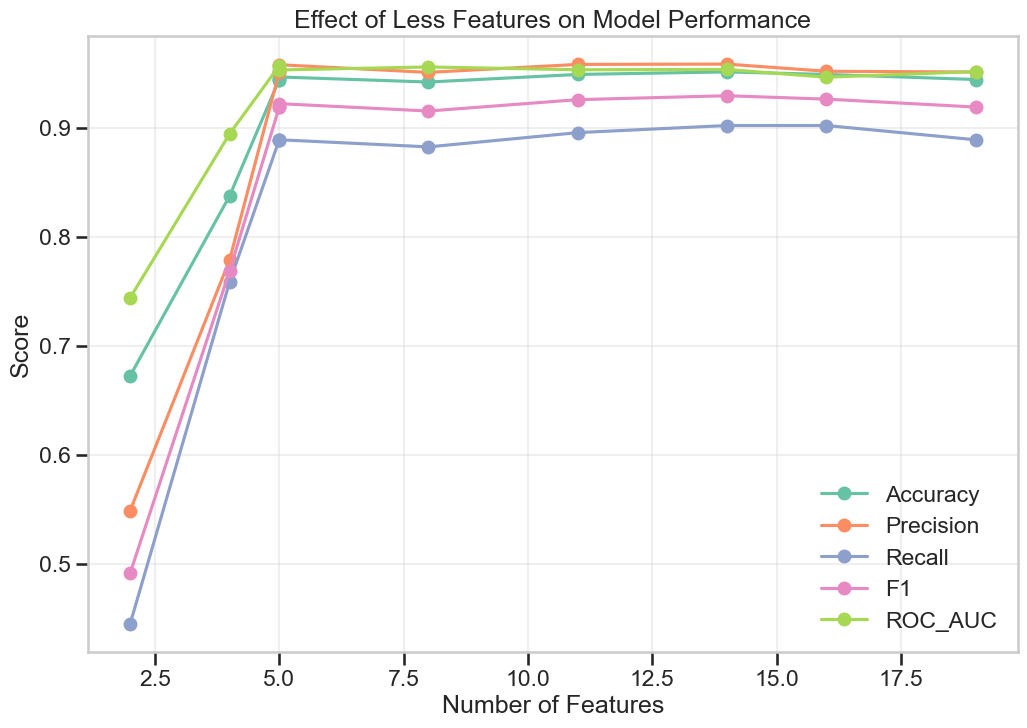
\includegraphics[width=0.5\textwidth]{figures/effect_less_features.png}
    \caption{Effect of Feature Deduction on Model Performance}
    \label{fig:feature_count}
\end{figure}

Results indicate that performance saturates around 5-7 features, suggesting that a small subset of key indicators can effectively predict Alzheimer's disease. This finding has important implications for clinical practice, where simpler models with fewer required measurements are preferable.

\section{Summary}
\label{sec:summary}

This study compared three classification methods for predicting Alzheimer's disease: Logistic Regression, Random Forest, and XGBoost. All models demonstrated strong performance, with XGBoost slightly outperforming the others. Feature importance analysis consistently identified cognitive assessments and behavioral indicators as the most predictive features across all models.

Feature selection using RFE identified an optimal subset of features that maintained or improved model performance while reducing complexity. The stacking ensemble model, which combined all three base models, achieved the highest overall performance.

Key findings include:
\begin{itemize}
    \item Cognitive assessments (MMSE, Functional Assessment, ADL) and behavioral indicators are the strongest predictors of Alzheimer's disease.
    \item A small subset of 5-7 features is sufficient for accurate prediction, with performance saturating beyond this point.
    \item Ensemble methods, particularly stacking, outperform individual models by leveraging their complementary strengths.
\end{itemize}

These findings suggest that machine learning models can effectively support clinical diagnosis of Alzheimer's disease using a relatively small set of key indicators. Future research could explore the temporal stability of these predictors and their utility in early detection.


\printbibliography

\end{document}